\NeedsTeXFormat{LaTeX2e}
\documentclass[fleqn,11pt]{article}

\usepackage[dvips,a4paper]{geometry}
\hoffset -1in
\voffset -1in
\setlength{\parskip}{1mm}
\setlength{\parindent}{0mm}
\setlength{\oddsidemargin}{20mm}
\setlength{\evensidemargin}{20mm}
\setlength{\topmargin}{20mm}
\setlength{\headheight}{0mm}
\setlength{\headsep}{0mm}
\setlength{\textwidth}{165mm}
\setlength{\textheight}{240mm}
\setlength{\footskip}{0mm}

\usepackage[english,english]{babel}
\usepackage[latin1]{inputenc}
\usepackage{graphicx}
\usepackage{amsmath,amssymb}
\usepackage{moreverb}
\usepackage{psfrag}
\usepackage[ps2pdf]{hyperref}
\usepackage{listings}
\usepackage{macros}

\graphicspath{{Figures/}}

\setcounter{tocdepth}{2}

\newcommand{\MBSim}{\href{http://mbsim.berlios.de}{\textsf{MBSim}}}
\newcommand{\OpenMBV}{\href{http://*.berlios.de}{\textsf{OpenMBV}}}
\newcommand{\FMatVec}{\href{http://fmatvec.berlios.de}{\textsf{FMatVec}}}
\newcommand{\HDF}{\href{http://www.hdfgroup.org/HDF5/}{\textsf{HDF5}}}

% document
\begin{document}
\title{\MBSim{} - A Kind (Of) Introduction}
\author{by \MBSim{} Development Team\\
  Mathias Bachmayer\\
  Bastian Esefeld\\
  Martin F\"org\\
  Markus Friedrich\\
  Robert Huber\\
  Thorsten Schindler\\
  Markus Schneider\\
  Roland Zander}
\date{28.07.2009}
\maketitle

\begin{abstract}
  This manual explains how to install \MBSim{} and introduces easy examples.
\end{abstract}

\noindent\hrulefill
\tableofcontents

%%%%%%%%%%%%%%%%%%%%%%%%%%%%%%%%%%%%%%%%%%%%%%%%%%%%%%%%%%%%%%%%%%%%%%%%%%%%%%%%
%%%%%%%%%%%%%%%%%%%%%%%%%%%%%%%%%%%%%%%%%%%%%%%%%%%%%%%%%%%%%%%%%%%%%%%%%%%%%%%%

\section{Introduction}
\MBSim{} is a simulation tool to analyse the dynamic phenomenons of dynamical systems. Its root is the modelling of nonsmooth multibody system explaining the program name \MBSim{}. The mathematical background has been developed over years at the Institute of Applied Mechanics of the Technische Universit\"at M\"unchen. The last summary concerning rigid body dynamics was given in the PhD thesis and the lecture of Martin F\"org~\cite{Foer09,Foer07}. The PhD thesis of Roland Zander~\cite{Zan09} introduces the theory of flexible bodies. Ref.~\cite{Zan08} shows an overview about the research at the institute in the last decades concerning nonsmooth mechanics. This reference also includes simulation results of academic and industrial examples. Extensions regarding hydraulics and signal processing as well as parallelisation and cosimulation are unique in the field of nonsmooth dynamical systems.\par
The goal of this introduction is to motivate the use of \MBSim{}. It shows the installation of the necessary program parts, describes basically its components and program flow and gives some examples. You find it in the Download section of the \MBSim{} webpage, where you can also find binary releases for Linux and Windows as well as~\cite{Zan08}. For more information, e.g. Doxygen description and current build status, visit the {\href{http://www4.amm.mw.tu-muenchen.de:8080/mbsim-env/}{\textsf{Central Build System}}}.


\section{Installation}
This section summarizes the necessary steps to install \MBSim{}.
%
\subsection{Where to find the source code}
The source code of \MBSim{} together with some examples, the necessary \FMatVec{} library, a \HDF{} wrapper for output and the visualisation program \OpenMBV{} can be found at \url{https://github.com} using git\footnote{GIT CHEAT SHEET: \url{https://training.github.com/kit/downloads/github-git-cheat-sheet.pdf}}. Everything is placed under \href{http://www.gnu.org/licenses/lgpl.html}{LGPL}\footnote{see file~\texttt{COPYING} in the root directory of the specific source code}.\par
%
\subsection{Installation procedures}
For the installation of the specific projects always the same \emph{procedures} have to be applied. They are summarized in the following.

\subsubsection{Installation}
\begin{itemize}
	\item \textsc{automake}:
	\begin{itemize}
		\item[] \begin{verbatim}autoreconf -fi\end{verbatim}
	\end{itemize}
	\item \textsc{configure}: 
	\begin{itemize}
		\item[] \begin{verbatim}./configure \end{verbatim}
    \item[] with defining a location for the installation 
                \begin{verbatim}--prefix=$HOME/.../Install\end{verbatim}
		\item[] possibly with project depending FLAGS which we find invoking \begin{verbatim}--help\end{verbatim} 
	\end{itemize}
	\item \textsc{install}
	\begin{itemize}	
		\item \begin{verbatim}make\end{verbatim}
		\item \begin{verbatim}make install\end{verbatim}
	\end{itemize}
\end{itemize}
All procedures belong to the GNU-Build-System (cf.~Sec.~\ref{sec:gnu}).

\subsubsection{Reinstallation/update}
The procedure \textsc{reinstall}
\begin{verbatim}
 make uninstall 
 make clean
 ./config.status --recheck
 make install
\end{verbatim}
newly installs a project with the same configure options used at the previous installation. These information are stored in the file config.status.\\ 
%
The procedure \textsc{update} is similar to the reinstallation:
\begin{verbatim}
 make uninstall 
 make clean
 git pull
 ./config.status --recheck
 make install
\end{verbatim}
For restoring a not-configured version of the project
\begin{verbatim}
 make maintainer-clean
\end{verbatim}
is used. After that \textsc{configure} has to be invoked.

\subsubsection{Uninstallation}
For uninstalling
\begin{verbatim}
 make uninstall
 make clean
\end{verbatim}
has to be called in all directories. If the files created by configure should be deleted, we type 
\begin{verbatim} 
 make distclean 
\end{verbatim} 
%
\begin{figure}[hbt]%
	\centering
    \footnotesize
    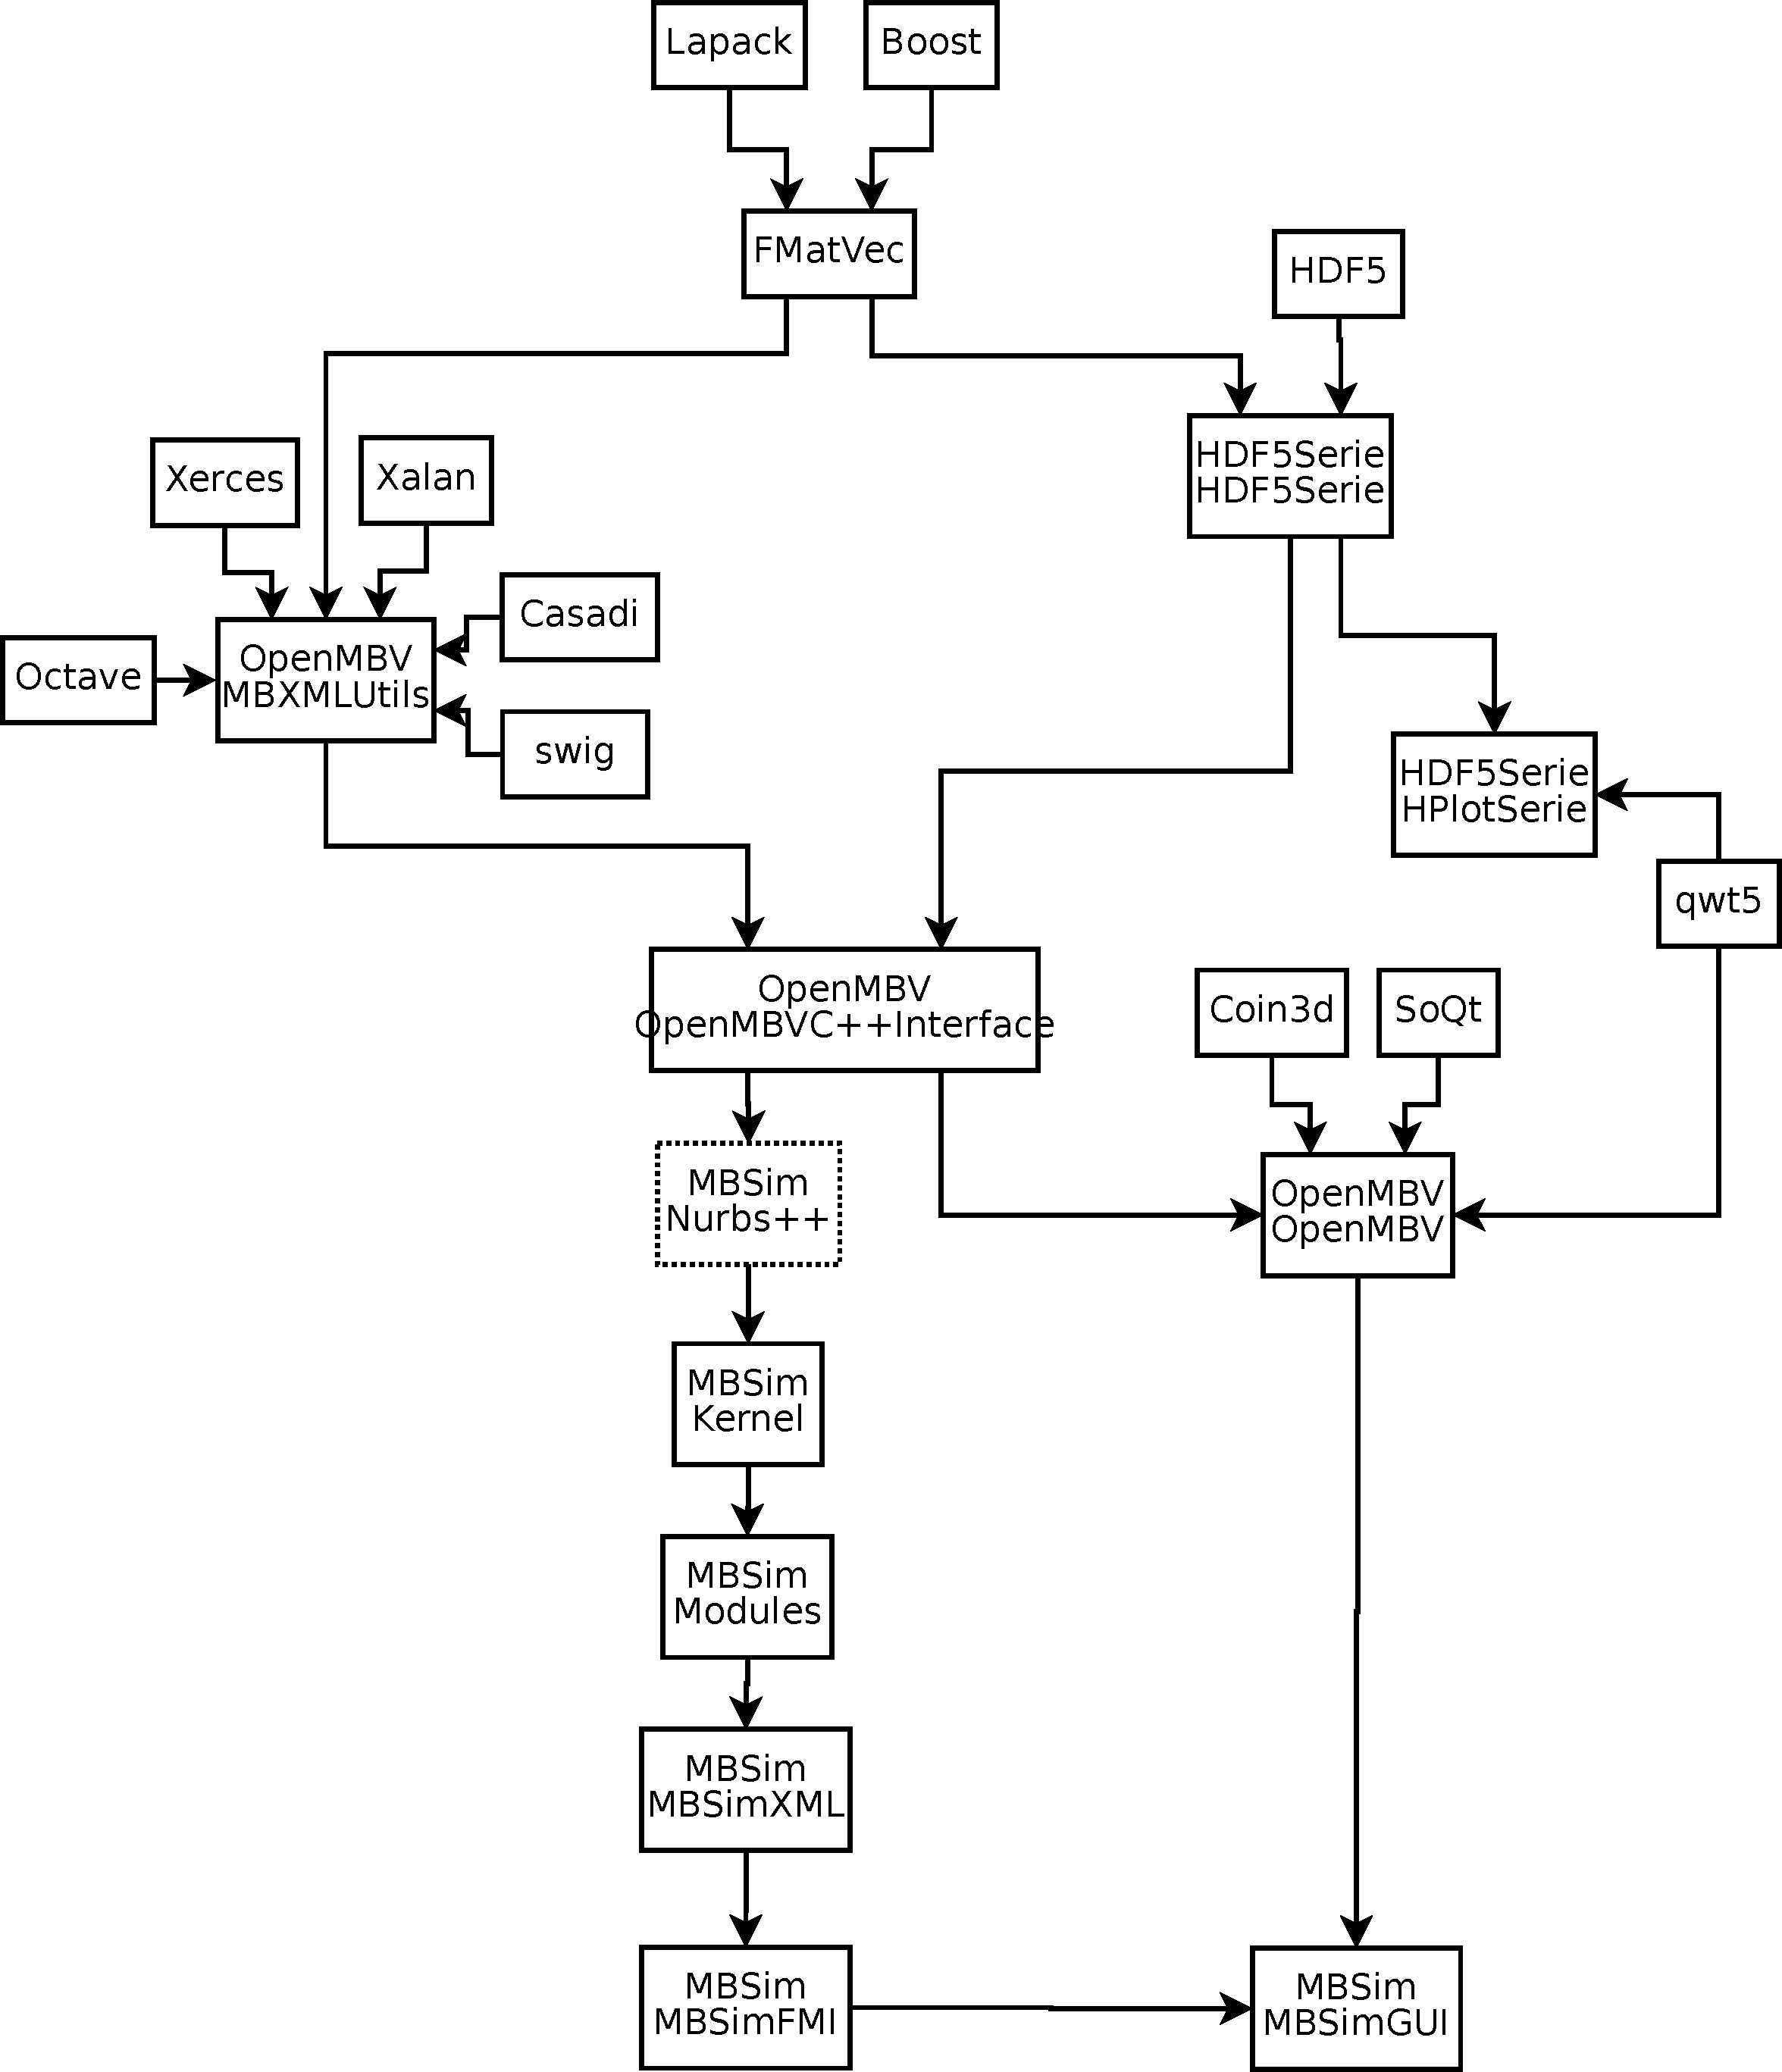
\includegraphics[width=0.95\hsize]{Figures/mbsim_install_flow.pdf}
    \caption{Installation flow for \MBSim{}}
    \label{fig:departure:mbsim:install_flow}
\end{figure}
%
\cleardoublepage
%
\subsection{Installation of the simulation framework\label{sec:install:simulation}}
It is assumed that a directory~\texttt{MBSim} and a directory \texttt{MBSim/Install} have been created in the \texttt{\$HOME} path of the Linux operating system. All projects depend on PKG package administration. The file \texttt{\$HOME/.bashrc} has to be extended with
\begin{verbatim}
 export PKG_CONFIG_PATH=
        "$HOME/MBSim/Install/lib/pkgconfig/:$PKG_CONFIG_PATH"
 export LD_LIBRARY_PATH=
        "$HOME/MBSim/Install/lib/:$LD_LIBRARY_PATH"
\end{verbatim}

\subsubsection{\FMatVec{}}
It is assumed that boost is installed. For the installation the following instructions have to be completed:
\begin{verbatim}
 cd $HOME/MBSim
 git clone https://github.com/mbsim-env/fmatvec.git
 cd $HOME/MBSim/fmatvec
\end{verbatim}
Continue with the procedure \textsc{automake}.\par
The procedure \textsc{configure} for dynamic compilation is used with
\begin{verbatim}
--prefix=$HOME/MBSim/Install
\end{verbatim}
The code can be compiled and installed with a Doxygen HTML class documentation by \texttt{make doc} and the procedure \textsc{install}.

\subsubsection{\HDFSerie}
%
\paragraph{\HDF}
\HDF{} is a hierarchical data format enabling the effective administration of plot and visualisation data. It can be downloaded as \textbf{source code} ("ALL Platforms") from \url{http://www.hdfgroup.org/HDF5/}, e.g. with version 1.8.15.\\
%
Change to \texttt{\$HOME/MBSim/hdf5}.\\
%
Use the procedure \textsc{configure} for dynamic compilation with
\begin{verbatim}
--prefix=$HOME/MBSim/Install
\end{verbatim}
and the additional FLAG
\begin{verbatim}
 --enable-cxx
\end{verbatim}
Compilation is done with the procedure \textsc{install}.
%
\paragraph{\HDFSerie}
It is assumed that \FMatVec{} is installed. \HDFSerie is available by
\begin{verbatim}
 cd $HOME/MBSim
 git clone https://github.com/mbsim-env/hdf5serie.git
\end{verbatim}
For having \MBSim{} creating \HDF{} files invoke
\begin{verbatim}
 cd $HOME/MBSim/HDF5Serie/hdf5serie
\end{verbatim}
as well as the procedures \textsc{automake, configure} for dynamic compilation with
\begin{verbatim}
--prefix=$HOME/MBSim/Install
\end{verbatim}
\texttt{make doc} and \textsc{install} for installation and creation of a Doxygen HTML class documentation.\\
%
Last, \texttt{.bashrc} can be extended with
\begin{verbatim}
alias h5lsserie="$HOME/MBSim/Install/bin/h5lsserie"
alias h5dumpserie="$HOME/MBSim/Install/bin/h5dumpserie"
\end{verbatim}
to gain overall access to the commands \texttt{h5lsserie} and \texttt{h5dumpserie}.

\subsubsection{\OpenMBV{}}
The installation for the simulation framework consists of three steps: first Casadi and the XMLUtils have to be installed, then \MBSim{} needs \textsf{OpenMBV-C++Interface} to create standard data for \OpenMBV{} using C++ programs. The source code is available by
\begin{verbatim}
 cd $HOME/MBSim
 git clone https://github.com/mbsim-env/openmbv.git
\end{verbatim}
%
\paragraph{Casadi}
For installing Casadi, take
\begin{verbatim}
  git clone https://github.com/casadi/casadi.git
\end{verbatim}
create a build-directory
\begin{verbatim}
  cd casadi, mkdir build, cd build
\end{verbatim}
and invoke
\begin{verbatim}
  cmake -DCMAKE_INSTALL_PREFIX=$HOME/MBSim/Install ..
\end{verbatim}
Proceed with
\begin{verbatim}
  make install
\end{verbatim}
%
\paragraph{XMLUtils}
It is assumed that \FMatVec{}, Octave, swig, Xerces, Xalan and Casadi are installed.
\begin{verbatim}
 cd $HOME/MBSim/OpenMBV/mbxmlutils
\end{verbatim} 
and use the procedures \textsc{automake}, \textsc{configure} for dynamic compilation with
\begin{verbatim}
--prefix=$HOME/MBSim/Install
\end{verbatim}
and \textsc{install} for installation of an independent XML preprocessor to parse and validate hierarchical XML-files.

\paragraph{OpenMBV-C++Interface}
It is assumed that \HDFSerie{} and XMLUtils are installed. Invoke
\begin{verbatim}
 cd $HOME/MBSim/OpenMBV/openmbvcppinterface
\end{verbatim} 
and the procedures \textsc{automake, configure} for dynamic compilation with
\begin{verbatim}
--prefix=$HOME/MBSim/Install
\end{verbatim}
Sometimes trouble with linking \emph{swig} occurs; in this case just set
\begin{verbatim}
--with-swigpath=/nope
\end{verbatim}
to some value such that \emph{swig} is not found on your system.\\
%
\texttt{make doc} and \textsc{install} for installation and creation of a Doxygen HTML class documentation. 
%
\subsubsection{\MBSim}
Necessary for the installation of \MBSim{} is OpenMBV-C++-Interface. For installation, one types
\begin{verbatim}
 cd $HOME/MBSim
 git clone https://github.com/mbsim-env/mbsim.git
\end{verbatim}
%
\paragraph{NURBS thirdparty package}
If you like, you can install the NURBS thirdparty package first, which is necessary for some examples. Invoke the procedures \textsc{automake, configure} for dynamic compilation with the prefix
\begin{verbatim}
--prefix=$HOME/MBSim/Install
\end{verbatim}
in \texttt{\$HOME/MBSim/mbsim/thirdparty/nurbs++}.
%
\paragraph{MBSim kernel}
Then proceed and invoke the procedures \textsc{automake, configure} for dynamic compilation with
\begin{verbatim}
--prefix=$HOME/MBSim/Install
\end{verbatim}
in \texttt{\$HOME/MBSim/mbsim/kernel}.\\
%
\texttt{make doc} and \textsc{install} to install the basic module and to create a Doxygen HTML class documentation. In
\begin{verbatim}
$HOME/MBSim/mbsim/kernel/xmldoc
\end{verbatim}
invoke \textsc{install} for an XML documentation in\\
\texttt{\$HOME/MBSim/Install/share/mbxmlutils/doc}.
%
\paragraph{Modules}
The following modules are available in MBSim:
%
\begin{itemize}
  \item mbsimControl
  \item mbsimHydraulics
  \item mbsimFlexibleBody
  \item mbsimElectronics
  \item mbsimPowerTrain
  \item mbsimInterface
\end{itemize}
%
The installation proceeds as follows:
\begin{verbatim}
  cd $HOME/MBSim/mbsim/modules/mbsimControl
\end{verbatim}
Invoke the procedures \textsc{automake, configure} for dynamic compilation with
\begin{verbatim}
--prefix=$HOME/MBSim/Install
\end{verbatim}
\texttt{make doc} and \textsc{install} to install the signal processing and control module and to create a Doxygen HTML class documentation. In 
\begin{verbatim}
  $HOME/MBSim/mbsim/modules/mbsimControl/xmldoc
\end{verbatim}
invoke \textsc{install} for an XML documentation in\\
\texttt{\$HOME/MBSim/Install/share/mbxmlutils/doc}.\\
%
Proceed in the same way for the other modules in the order as given above.
%
\paragraph{MBSimXML}
MBSimXML offers the possibility to define mechanical systems with XML.
\begin{verbatim}
  cd $HOME/MBSim/mbsim/mbsimxml
\end{verbatim}
Invoke the procedures \textsc{automake, configure} for dynamic compilation with
\begin{verbatim}
  --prefix=$HOME/MBSim/Install
\end{verbatim}
and \textsc{install} to install the XML module which contains an executable to invoke the preprocessor. In
\begin{verbatim}
  $HOME/MBSim/mbsim/mbsimxml/xmldoc
\end{verbatim}
invoke \textsc{install} for an XML documentation in\\
\texttt{\$HOME/MBSim/Install/share/mbxmlutils/doc}.
%
\paragraph{MBSimFMI}
MBSimFMI gives an interface for model export. Proceed as follows:
\begin{verbatim}
  cd $HOME/MBSim/mbsim/mbsimfmi
\end{verbatim}
Invoke the procedures \textsc{automake, configure} for dynamic compilation with
\begin{verbatim}
  --prefix=$HOME/MBSim/Install
\end{verbatim}
and \textsc{install}.
%
\paragraph{MBSimGUI}
MBSimGUI offers a GUI for \MBSim{}. If we have installed \OpenMBV{}, we can install it.
\begin{verbatim}
  cd $HOME/MBSim/mbsim/mbsimgui
\end{verbatim}
Invoke the procedures \textsc{automake, configure} for dynamic compilation with
\begin{verbatim}
  --prefix=$HOME/MBSim/Install
\end{verbatim}
and \textsc{install}.

\subsubsection{Examples}
The examples are used for testing successful installation. There are two possibilities:
\begin{enumerate}
\item Change to the specific directory \texttt{\$HOME/MBSim/mbsim/examples/*} and type \texttt{make} to create an executable. The simulation starts with the command~\texttt{./main}. The results are visualised with the command~\texttt{openmbv} and plotted with~\texttt{h5plotserie} after having installed the visualisation framework (Sec.~\ref{sec:install:visualisation} and \ref{sec:plot}).
\item Use the script \texttt{python runexamples.py} in \texttt{\$HOME/MBSim/mbsim/examples} to compile, run and test each example. See \texttt{python runexamples.py --help} for additional information.
\end{enumerate}
%
\subsection{Installation of the visualisation framework\label{sec:install:visualisation}}
It is assumed, that a directory~\texttt{OpenMBV} and a directory \texttt{OpenMBV/Install} has been created in the \texttt{\$HOME} path of the Linux operating system. The necessary software is described in Sec.~\ref{sec:third_party}). This subsection describes a \textbf{static} compilation, therefore the additional FLAG have to be used in each step
\begin{verbatim}
  --disable-shared --enable-static
\end{verbatim}

\subsubsection{\HDF}
Install \HDF{} and the \HDFSerie{} as described in Sec.~\ref{sec:install:simulation} but in the directory \texttt{OpenMBV} and using a static compilation. For plotting of \HDF{} files it is assumed that Qwt with version 5 is installed. Invoke 
\begin{verbatim}
  cd $HOME/OpenMBV/HDF5Serie/h5plotserie
\end{verbatim}
as well as the procedures \textsc{automake, configure} for static compilation, \texttt{make doc} and \textsc{install} for installation and creation of a Doxygen HTML class documentation. \texttt{.bashrc} can be extended with
\begin{verbatim}
  alias h5plotserie="$HOME/OpenMBV/Install/bin/h5plotserie"
\end{verbatim}
to gain overall access to the command \texttt{h5plotserie}.

\subsubsection{\OpenMBV{}}
\paragraph{XML Utils}
Install XML Utils as described in Sec.~\ref{sec:install:simulation} but in the directory \texttt{OpenMBV} and using a static compilation.

\paragraph{OpenMBV-C++Interface}
Install OpenMBV-C++Interface as described in Sec.~\ref{sec:install:simulation} but in the directory \texttt{OpenMBV} and using a static compilation.

\paragraph{\OpenMBV{}}
For the installation of a static visualisation using always the newest source files it is assumed that Coin3d, MBXMLUtils, \HDFSerie, SoQt, Qwt with version 5 are installed. With
\begin{verbatim}
  cd $HOME/OpenMBV/OpenMBV/openmbv
\end{verbatim} 
and the procedures \textsc{automake, configure} for static compilation. \texttt{make doc} and \textsc{install} complete the installation of the viewer with an Doxygen HTML class documentation. \texttt{.bashrc} can be extended with
\begin{verbatim}
  alias openmbv="$HOME/OpenMBV/Install/bin/openmbv"
\end{verbatim}
to gain overall access to the command \texttt{openmbv}.

\section{\MBSim - Program Overview}
\MBSim{} is written in the object-orientated programming language C++. 

Fig.~\ref{fig:objects} shows a class diagram.
\begin{figure}
	\centering
  	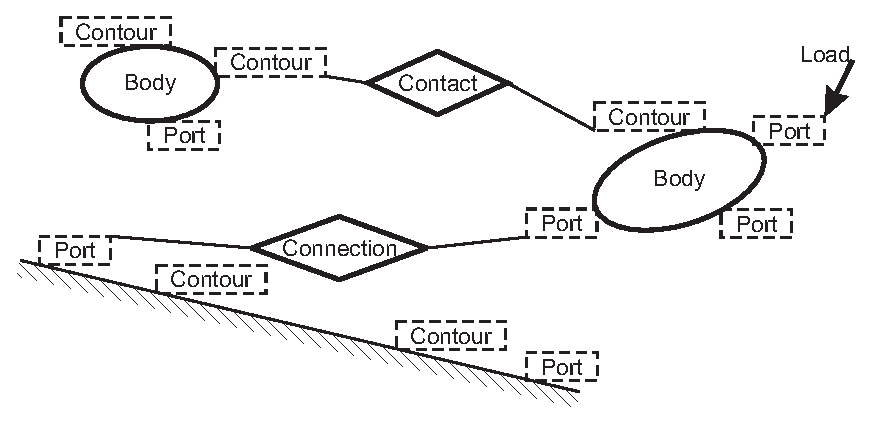
\includegraphics[width=12cm]{Figures/objectorientationMBSim.eps} % TODO
  	\caption{object structure in \MBSim}
  	\label{fig:objects}
\end{figure}
Exemplary this is a dynamical system with environment and two bodies. Indicated are interconnections due to contacts and joints as well as an external load.\par
A body is defined with respect to its generalised coordinates and velocities, contacts between contours and joints between frames may be rigid or flexible also including friction. The definition of loads might include arbitrary functional descriptions.

\subsection{Description of the Components}
The following classes can be used for modelling and simulating dynamical systems in \MBSim{}.

\subsubsection{DynamicSystem and DynamicSystemSolver}
Hierarchically frames, bodies and interconnections belong to \texttt{DynamicSystem}s. For their definitions a canonic stationary frame \texttt{"I"} always exists. The top-most \texttt{DynamicSystem} is called \texttt{DynamicSystemSolver}. It also represents the interface to the integration schemes and allows the setting of environment variables (e.g. gravitation). Important settings: \emph{setReorganizeHierarchy} enforces the automatic creation of an invisible tree structures for the simulation process

\subsubsection{Frames}
\texttt{Frame}s are a basic concept in \MBSim{} to define an interface for kinematic and kinetic expressions using a frame recursive relationship. Important settings: \emph{enableOpenMBV} enabling visualisation

\subsubsection{Rigid Bodies}
A \texttt{RigidBody} is based on a predefined frame \texttt{"C"} in the centre of gravity. This frame can e.g. be used to describe further frames at rigid bodies. Then, one frame for kinematics has to be chosen being updated with respect to a reference frame as well as the individual degree of freedom of the \texttt{RigidBody} or its constrained relative motion. Both absolute and relative kinematical structures are canonically given by this frame recursion depending on the properties of the reference. The drawback of this general description is a time-dependent mass-matrix. If there is a frame given tree structure a \texttt{Tree} for the kinematical evaluations is defined automatically.\\
Important settings: \emph{setMass}, \emph{setInertiaTensor}, \emph{setFrameOfReference}, \emph{setFrameForKinematics}, \emph{setTranslation} describing the translational degrees of freedom, \emph{setRotation} describing the rotational degrees of freedom, \emph{setOpenMBVRigidBody} to enable visualisation\\
Initial values: are given by the reference frame

\subsubsection{Flexible Bodies}
The equations of motion of a \texttt{FlexibleBody} is at the moment always derived with respect to a stationary frame. So, flexible bodies can only be used as root but not as leave in a recursive tree structure. The following flexible bodies are available. 

\begin{itemize}
%\item \emph{BodyFlexible1s01Torsion}
%\item \emph{BodyFlexible1s21ANCF} 2D-Balken mit Absolute Nodal Coordinate Formulation
\item[] \texttt{BodyFlexible1s21RCM}\\
  planar beam using redundant coordinate methode with three coordinates per finite element node, translation  $x$, $y$ and rotation $\gamma$, as well as two additional bending deflections $c_1$, $c_2$
\item[] \texttt{BodyFlexible1s33RCM}\\
  spatial beam using redundant coordinate methode with six coordinates per finite element node, translation  $x$, $y$, $z$ and reversed Cardan rotation $\alpha$, $\beta$, $\gamma$, as well as four additional bending deflections $c_1$, $c_2$, $c_3$, $c_4$
%\item \emph{BodyFlexible1s23BTA} Biege-Torsions-Welle (5-Koordinaten pro Knoten $\alpha$, $y$, $\gamma$, $z$, $\beta$ im jeweils mit $\alpha$ mitdrehenden KOSY)
%\item \emph{BodyFlexibleLinearExternal}
\end{itemize}

\subsubsection{LinkMechanics}
Mechanical links represent interconnections between mechanical bodies.

\paragraph{Actuators}
An \texttt{Actuator} connects two frames using a predefined control function.

\paragraph{Joints}
\texttt{Joint}s connect two frames with the force laws depending on the ideal normal relative kinematics. The constitutive law has to be chosen for the calculation of the force parameter. 
Important settings: \emph{setForceDirection}, \emph{setMomentDirection}, \emph{setForceLaw} (acceleration level), \emph{setImpactForceLaw} (velocity level)

\paragraph{Contacts and Impacts}
Contacts and impacts are managed by \texttt{Contact}.
Important settings: \emph{setContactForceLaw}, \emph{setContactImpactLaw}, \emph{setFrictionForceLaw}, \emph{setFrictionImpactLaw}, \emph{setContactKinematics} \par 
The relative kinematics is defined between \texttt{Contour} classes. Thereby kinematically there might be a finite number of possible contact points; for the evaluation of force laws a decision rule has to be implemented. On velocity level the contact kinematics is independent of the specific contour. For the calculations on position level the following contours are available.
\begin{itemize}
\item[] \texttt{CircleHollow}\\
    one dimensional sphere with contact from inside 
\item[] \texttt{CircleSolid}\\
    one dimensional sphere with contact from outside 
\item[] \texttt{FlexibleBand}\\
    flexible contour describing a band in a certain distance and direction of a neutral fibre
\item[] \texttt{Frustum}\\
    frustum with its axis given by the second column of the contour reference frame
\item[] \texttt{Line}\\
    affine one dimensional space 
\item[] \texttt{Plane}\\
    affine two dimensional surface
\item[] \texttt{Point}\\
    most primitive rigid contour
\item[] \texttt{Sphere}\\
    two dimensional sphere
\end{itemize}

Available contact kinematics on position level:
\begin{itemize}
\item[] \texttt{CircleSolidLine}
\item[] \texttt{PointLine}
\item[] \texttt{PointFrustum}
\item[] \texttt{PointPlane}
\item[] \texttt{PointFlexibleBand}
\item[] \texttt{SpherePlane}
\end{itemize}

\paragraph{Constitutive Laws}
Concerning the constitutive laws it is distinguished between contact laws on acceleration and impact laws on velocity level. Further, both flexible and rigid laws in normal and tangential direction are available.\footnote{Modelling hint: There are contradictions between energy conservation in normal direction and dissipation due to friction when combining these features.})\par

\paragraph{Conventions}
For modelling own contact kinematics and constitutive laws some conventions are important.
\begin{itemize}
\item contact kinematics\\
    \texttt{updateg} should define the normal distance, the possible contact locations and trihedral orientations, \texttt{updatewb} are nonlinear kinematic terms
\item accompanying contour trihedral\\
    the first column is the outward pointing normal, 
\end{itemize}

\subsubsection{Integration Schemes}
Available integration schemes:
\begin{itemize}
\item[] \texttt{DOPRI5Integrator}\\
    Dormand-Prince one-step integration scheme of order 5 for nonstiff ODE with step size control
\item[] \texttt{RADAU5Integrator}\\
    one-step integration scheme of order 5 for stiff ODE with step size control
\item[] \texttt{TimeSteppingIntegrator}\\
    one-step semi-implicit integration scheme of order 1 for nonstiff MDE
\item[] \texttt{ThetaTimeSteppingIntegrator}\\
    one-step integration scheme of order 1 for nonstiff with $\Theta=0$ and stiff with $\Theta\in\left(0,1\right] $MDE
\end{itemize}
%DAEs behandeln \emph{RADAU5DAEIntegrator}, \emph{DASKRIntegrator} und \emph{DASPKIntegrator}. Dar\"uberhinaus gibt es noch \emph{RKSuite}, \emph{LSODAR} (Mehrschrittverfahren steif/nicht steif) und \emph{LSODE}.  oder der allgemeinere \emph{ThetaTimeSteppingIntegrator} mit konstanter Schrittweitenvorgabe angewendet werden. \emph{TimeSteppingSSCIntegrator} implementiert f�r den semi-impliziten Fall eine Schrittweitensteuerung und \emph{DAETSIntegrator} liefert eine Kopplung zwischen TimeStepping und Dassl. Bei letzteren muss der Befehl \texttt{setSolver} vor der Initialisierung des MBS durchgef\"uhrt werden. Folgende M\"oglichkeiten stehen zur Wahl:

Available constraint equation solution schemes:
\begin{itemize}
\item[] \texttt{GaussSeidel}\\
    Gauss-Seidel solution scheme for piecewise linear systems (planar Coulomb friction)
\item[] \texttt{FixedPointSingle}\\
    Gauss-Seidel solution scheme with fixed point search and relaxation strategy for spatial Coulomb friction
\item[] \texttt{RootFinding}\\
    damped and globalised Newton scheme for spatial Coulomb friction
\end{itemize}
%\begin{itemize}
%\item Invertierbare Gleichungssysteme (GS) mit nur bilateralen Bindungen\\
%\emph{LinearEquations}: Cholesky-Verfahren
%
%
%\item Nichtlineare GS (3D-Coulomb-Reibung)\\
%  (\emph{setStrategy} mit \emph{local}/\emph{global})\\
%\emph{FixedPointTotal}: Jacobi-Verfahren mit Fixpunktsuche und R-Faktor-Strategie (verh\"alt sich zumeist schlechter als \emph{FixedPointSingle})\\  
%\emph{RootFinding}: 
%  R-Faktor-Strategie (unstetige Jacobi-Matrix) und f\"ur unterbestimmte LGS ausw\"ahlbarer \emph{setLinalg} (LUDecomposition, LevenbergMarquardt, PseudoInverse) (f\"ur schlecht konditionierte Dylassus-Matrix meistens am besten)
%\end{itemize}
%Der Befehl \emph{stopifnoConvergence(\texttt{true},\texttt{true})} zwingt den Integrator abzubrechen, falls keine Konvergenz vorliegt, und die Kontaktsituation auszugeben.
%

\subsection{Program Flow}
Conceptionally the program flow is defined by the election of the integration scheme. It can always be stopped using \texttt{Ctrl-C} also enforcing the closing of the plot functionality. With
\begin{verbatim}
kill -USR2 <PID of simulation thread>
\end{verbatim}
a flush of the plot routine is asked for.

\subsubsection{Timestepping Integration}
Timestepping integration solves the whole equations of the system including the contacts on velocity level with fixed time step size. In detail one has the following work flow.
\begin{enumerate}
\item $\text{\texttt{DS::plot}}\left(t,\vq,\vu\right)$
\item $\vq\leftarrow\vq+\text{\texttt{DS::deltaq}}\left(t,\vq,\vu\right)$
\item $t\leftarrow t+\Delta t$
\item $\text{\texttt{DS::update}}\left(t,\vq,\vu\right)$
    \begin{enumerate}
    \item[]\texttt{DS::updateStateDependentVariables}\\
      update variables depending on the generalised state and the structure of the system with one independent group and several trees
    \item[]\texttt{DS::updateg}
      \begin{itemize}
      \item update of the relative position kinematics independent of the system structure using the order
      \begin{align*}
        \text{\texttt{Link}}\rightarrow\text{\texttt{LinkMechanics}}\rightarrow\text{\texttt{Joint}, \texttt{Contact}, \texttt{Actuator}}\rightarrow\text{\texttt{ContactKinematics}}
      \end{align*}
      \item several contacts points are possible from the kinematical point of view, whereby the maximum number is calculated in \texttt{ContactKinematics}\\
      \item conventions in the contact frame matrix:
        \begin{itemize}
        \item frames are cartesian
        \item first column is the outpointing normal
        \item second column sign is different for the two contacting bodies 
        \end{itemize}
      \end{itemize}
    \item[]\texttt{DS::checkActiveg}
      \begin{itemize}
      \item determine the state of the relative kinematics concerning the activity of links
      \item redefine global memory references using indices and indents
      \end{itemize}
    \item[]\texttt{DS::updategd}
      \begin{itemize}
      \item update of the relative velocity kinematics independent of the system structure
      \item can be done in the child classes of \texttt{LinkMechanics}
      \end{itemize}
    \item[]\texttt{DS::updateT}\\
      updates the linear transformation matrix $\dot{\vq}=\vT\vu$ independent of the system structure
    \item[]\texttt{updateJacobians}\\
      updates the \textsc{Jacobians} for projecting forces in generalised directions dependent on the system structure
    \item[]\texttt{updateh}\\
      updates the right hand sides with the possibility to account for internal forces of \texttt{objects} and external forces of \texttt{links} independent of the system structure
    \item[]\texttt{updateM}\\
      updates the mass matrix independent of the system structure
    \item[]\texttt{facLLM}
      \begin{itemize}
      \item computes the \textsc{Cholesky} decomposition of the mass matrix dependent on the system structure
      \item \texttt{group} calculates the matrix inverse locally per object
      \item \texttt{tree} calculates the matrix inverse globally
      \end{itemize}
    \item[]\texttt{updateW}\\
      updates the \textsc{Jacobian} between in general set-valued \texttt{link}-force parameters and generalised coordinates
    \item[]\texttt{updateV}
      \begin{itemize}
      \item the decomposition of the in general set-valued \texttt{link}-forces
      \begin{align*}
      \vW\vlambda=\vW_N\vlambda_N+\vW_T\vlambda_T
      \end{align*}
      in a normal and tangential part allows to separate the single-valued slip case
      \item for affected \texttt{links} it is
      \begin{align*}
      \tilde{\vW}\tilde{\vlambda}=\left(\tilde{\vW}_N+\mu\tilde{\vW}_T\right)\tilde{\vlambda}_N=\tilde{\vV}\tilde{\vlambda}_N\ .
      \end{align*}
      \item altogether this is a reduction of the set-valued equations being expressed by the projection
      \begin{align*}
      \vV\vlambda^{*}\ .
      \end{align*}
      \end{itemize}
    \item[]\texttt{updateG}
      \begin{itemize}
      \item the force action matrix
      \begin{align*}
      \vG=\vW^T\vM^{-1}\vV
      \end{align*}
      must be calculated by the most global view, namely the \texttt{DynamicSystemSolver}
      \item the size of $\vG$ is reduced due to the introduction of $\vV$ but is non-symmetric
      \item for a time-stepping scheme it is $\vV=\vW$
      \end{itemize}
    \end{enumerate}
\item $\text{\texttt{DS::solveImpacts}}\left(t,\vq,\vu\right)$
    \begin{itemize}
    \item the constrained equations are solved on velocity level using sparse matrix structures (cf.~\cite[MKL sparse matrix storage format]{Intel08})
    \item block structures are not evaluated
    \end{itemize}
\item $\vu\leftarrow\vu+\text{\texttt{DS::deltau}}$
\item $\vx\leftarrow\vx+\text{\texttt{DS::deltax}}$
\item \texttt{DS::projectGeneralizedPositions}
\end{enumerate}

\subsubsection{Event-Driven Integration}
Currently, \texttt{LSODAR} is the only event-driven integrator with automatic switch between stiff and non-stiff equations.
\begin{enumerate}
\item \texttt{DS::computeInitialCondition}\\
    checks for system configuration and creates the necessary contact container
\item $\text{\texttt{DS::plot}}\left(t,\vq\right)$
\item \texttt{DLSODAR} 
    \begin{enumerate}
    \item[]$\text{\texttt{DS::zdot}}\left(t,\vq,\vu\right)$ is available for standard and inverse kinetics calculations
      \begin{itemize}
      \item \texttt{wb} means $\bar{w}$ and describes the acceleration terms in the constraint kinematics
      \item \texttt{computeConstraintForces} uses a least square algorithm to solve the Delassus equations, assume $Ax=b$ with a $m\times n$ full-rank matrix $A$, then there are two cases
        \begin{itemize}
        \item $m\geq n$ (skinny) can always be solved by $\left\|Ax-b\right\|\rightarrow\min$ and so by SVD\\
          analytically the solution is given by the normal equations $x=\left(A^TA\right)^{-1}A^Tb$
        \item $m<n$ (fat) has an infinite dimensional solution space, one has to pick one solution\\
          $\left\|x\right\|\rightarrow\min,\ Ax=b$ which is analytically given by $x=A^T\left(A^TA\right)^{-1}b$, again numerically a SVD solves the problem most efficiently
        \end{itemize}
      \end{itemize}
    \item[]\texttt{DS::getsv} the stop vector defines the root function concerning contacts and stick-slip-transitions for the DAE solver
      \begin{itemize}
      \item it can be only set by \texttt{Link}
      \item contains kinematics for not-active directions and kinetics for active directions
      \item the last entry is used for position and velocity projections
      \end{itemize}
    \end{enumerate}
\item \texttt{DS::shift} is invoked, if there is a sign change in the stop vector
    \begin{itemize}
      \item drift compensation if indicated by stop vector
      \item project to slighly positive gaps to avoid instantaneous appearance of new shift point
      \item[] \texttt{updateCondition} should impact or differential equations be solved, after earlier mentioned reconfiguring
      \item case studies
        \begin{itemize}
        \item[] \texttt{impact} has highest priority and changes overall configuration
        \item[] \texttt{impact} requires \texttt{D::checkAllgd} because of possible slip-stick transition
        \item no difference between $\Lambda$ and $\lambda$
        \item \texttt{gdn} means $\dot{g}^{+}$
        \item[] \texttt{impact} involves new configuration and so also the equations of motion have to be solved
        \item \texttt{checkActivegdd} has to be done with the same tolerance like in the nonlinear equations solver
        \item[] \texttt{gActive} means a contact is closed
        \item[] \texttt{gdActive} means a contact remains closed
        \end{itemize}
    \end{itemize}
\end{enumerate}

%%------------------------------------------------------------ SUBSECTION --
\subsection{Plot Routines}\label{sec:plot}

\subsubsection{Usage}
The result of a simulation with \MBSim{} are a \texttt{mbsim.h5} file for plot analysis as well as \texttt{ombv.h5} and \texttt{ombv.xml} files for visualisation. Additionally there is information concerning the integrator in \texttt{*.plt} and \texttt{*.sum} files; for visualisation \texttt{*.iv} files might appear.\\
For getting data from \MBSim{} a \HDF{} wrapper is used. Viewing the multibody system parts can be done with
\begin{verbatim}
    h5lsserie <h5-file>
\end{verbatim}
Several possible options are explained by typing \texttt{-h}:
\begin{enumerate}
\item[\texttt{-d}] shows the description of the data to plot\\
\item[\texttt{-l}] shows the column labels of the data to plot\\
\item[\texttt{-f}] follows external links in a set of \HDF{}-files to avoid redundant data (\HDF{} is possible per DynamicSystem)
\end{enumerate}
The specific names in \HDF{} format are specialised by reading from right to left. The url to specific data is given by a path and can be used in
\begin{verbatim}
    h5dumpserie <path>
\end{verbatim}
The column one is interested in is declared using a colon. Also several columns can be appended, whereby shorter ones are enlarged by \texttt{nan} entries. Altogether, it is possible to use the dump by
\begin{verbatim}
    gnuplot "<dump" u *:* w l
\end{verbatim}
or in \textsf{MatLab} by
\begin{verbatim}
    h5dump('<path>')
\end{verbatim}
A convenient tool for analysing data is given by
\begin{verbatim}
    h5plotserie <h5-file>
\end{verbatim}
The usage is quite canonic and documented in the online help. Interesting features are
\begin{itemize}
\item superimposing graphs by \texttt{<shift>}
\item plotting labels by \texttt{<ctrl>}
\item disabling graphs by double click
\end{itemize}

\subsubsection{Implementation}
In \MBSim{} plotting is done using \texttt{plotFeatures} being defined in \texttt{element.h} and set in \texttt{dynamic\_system\_solver.cc}. One plot-file comprises time-series of rowvectors with the same data type in all entries.


\section{Examples}

%%------------------------------------------------------------ SUBSECTION ---------------------
\subsection{Example: One-Mass-Oscillator With Recursive Structure and Impact}

\hspace*{0.2\hsize}
  \psfrag{x} [cc][cc]{$x$}
  \psfrag{K} [lc][lc]{Body}
  \psfrag{m} [cc][cc]{$m$}
  \psfrag{c} [cc][cc]{Spring $c$}
  \psfrag{S} [cc][cc]{$S$}
  \psfrag{K} [lc][lc]{Body with COG}
  \psfrag{pb}[lc][lc]{Frame on Body}
  \psfrag{pe}[lc][lc]{Frame on Environment}
  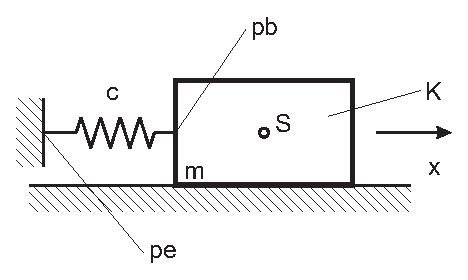
\includegraphics[width=0.45\hsize]{one_mass_oscillator}

%%------------------------------------------------------------ SUBSUBSECTION ---------------------
\subsubsection{Physics - system}

\paragraph{Header}

\listinginput{1}{C++/system.h}

\begin{tabular}{r|p{0.85\hsize}}
  1,2,13 & avoids including Header more than once\\
  4,5  & \emph{includes}\\
  7 & class definition for one mass oscillator, which is derived by \texttt{DynamicSystemSolver} without additional functionality\\
  9 & constructor
\end{tabular}

%------------------------------------------------------------
\paragraph{Source}

\listinginput{1}{C++/system.cc}

%%------------------------------------------------------------ SUBSUBSECTION ---------------------
\subsubsection{Time integration -- main}

\listinginput{1}{C++/main.cc}

%%------------------------------------------------------------ SUBSUBSECTION ---------------------
\subsubsection{Makefile} \enlargethispage{5mm}
The building process of a program is controlled by a Makefile:
\listinginput{1}{C++/Makefile}

%%--------------------------------------------------------------- SUBSECTION --
\subsection{2D-Slider Crank Mechanism}
Use the following plan.
\begin{enumerate}
\item rigid bodies with
\begin{itemize}
\item \emph{RigidBody} for crank, pistin and block
\item mass/ length/ width/ inertia tensor
\item Jacobian matrices (translation / rotation)
\item reference frames
\item \OpenMBV{}-bodies (probably one needs an additional translation as \OpenMBV{}-bodies sometimes use another reference)
\end{itemize}

\item elastic connecting rod with
\begin{itemize}
\item \emph{FlexibleBody1s21RCM}
\item length/ width / height (cross-sectional area) / Young's modulus (10e8)/ area moment of inertia / density/ damping
\item number of finite elements
\item reference frames
\item initial generalised coordinates
\end{itemize}

\item frames/ contours in body coordinate system
\item link definition
\item external loads
\item add to dynamic system solver
\item integrator / time step size
\end{enumerate}

%%--------------------------------------------------------------- SUBSECTION --
\subsection{3D-Slider Crank Mechanism}
Use the following plan.
\begin{enumerate}
\item rigid bodies with
\begin{itemize}
\item \emph{RigidBody} for crank, connecting rod, piston and block
\item mass/ length/ width / inertia tensor
\item Jacobian matrices (translation / rotation)
\item reference frames
\item \OpenMBV{}-bodies
\end{itemize}

\item frames / contours in body coordinate system
\item link definition
\item external loads
\item add to dynamic system solver
\item integrator / time step size
\end{enumerate}



\appendix
\section{Trouble-Shooting}
\subsection{Path Information}
After recognising difficulties concerning path information mistakes in the objects should be ruled out by \texttt{make clean}. Then, path information in \texttt{.bashrc} and finally in the affected \texttt{.pc}-files should be checked. The location of the \texttt{.pc}-files can be found by
\begin{verbatim}
pkg-config --cflags mbsim
pkg-config --libs mbsim
\end{verbatim}

\section{\MBSim{} - Coding Standard}
In the following the Coding standards of \MBSim{} and the associated projects is defined.
\listinginput{1}{mbsimcodingstandard.h}


%%%%%%%%%%%%%%%%%%%%%%%%%%%%%%%%%%%%%%%%%%%%%%%%%%%%%%%%%%%%%%%%%%%%%%%%%%%%%%%%
%%%%%%%%%%%%%%%%%%%%%%%%%%%%%%%%%%%%%%%%%%%%%%%%%%%%%%%%%%%%%%%%%%%%%%%%%%%%%%%%

\bibliographystyle{plain}
\bibliography{Literatur}
\end{document}

